%%% Local Variables:
%%% TeX-command-extra-options: "-shell-escape"
%%% End:

\section{Pipeline and CI}

\begin{frame}
\begin{figure}[ht]
  \caption{diagram of different projects}
  \centering
  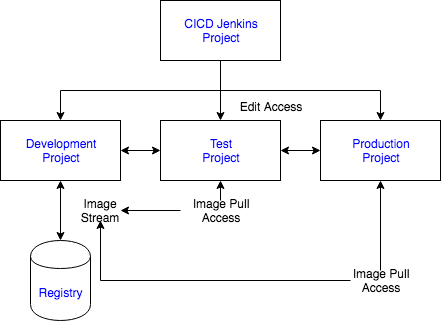
\includegraphics[scale=0.6]{ProjectPipelineDiagram.png}
  \label{fig:ProjectPipelineDiagram}
\end{figure}
\end{frame}

\begin{frame}
  \begin{itemize}
  \item Project CICD Containing our Jenkins instance
  \item Development For building and developing our application images
  \item Testing For testing our application
  \item Production Hosting our production application
  \end{itemize}
\end{frame}

\begin{frame}[fragile]
  \frametitle{Create Projects}
  \begin{bashcode}
    $ oc login -u developer -p developer
    $ oc new-project cicd --display-name='CICD Jenkins' \
    --description='CICD Jenkins'
    $ oc new-project development \
    --display-name='Development' --description='Development'
    $ oc new-project testing --display-name='Testing' \
    --description='Testing'
    $ oc new-project production --display-name='Production' \
    --description='Production'
  \end{bashcode}
\end{frame}

\begin{frame}[fragile]
  \frametitle{RBAC}
  
  \begin{bashcode}
    $ oc policy add-role-to-user edit \
    system:serviceaccount:cicd:jenkins -n development
    $ oc policy add-role-to-user edit \
    system:serviceaccount:cicd:jenkins -n testing
    $ oc policy add-role-to-user edit \
    system:serviceaccount:cicd:jenkins -n production
  \end{bashcode}
\end{frame}

\begin{frame}[fragile]
  \frametitle{RBAC}
  \begin{bashcode}
    $ oc policy add-role-to-group system:image-puller \
    system:serviceaccounts:testing -n development
    $ oc policy add-role-to-group system:image-puller \
    system:serviceaccounts:production -n development
  \end{bashcode}
\end{frame}


\subsection{Deploy Jenkins and Our Pipeline Definition}

\begin{frame}[fragile]
  \frametitle{Jenkins}
  Deploy a Jenkins ephemeral instance in \textit{cicd} project
  \begin{bashcode}
    $ oc project cicd
    $ oc new-app --template=openshift/jenkins-persistent
    $ oc status
  \end{bashcode}
  Let's create the pipeline itself.
  \begin{bashcode}
    $ oc create -n cicd -f \
    https://raw.githubusercontent.com/devops-with-openshift\
    /pipeline-configs/master/pipeline.yaml
  \end{bashcode}
\end{frame}

\subsection{Deploy Our Sample Application}
\begin{frame}[fragile]
  \frametitle{Jenkins}
  \begin{bashcode}
    $ oc project development
    $ oc create new-app --name=cdnapi \
    https://github.com/gandalf-the-white/faye.git
    $ oc expose svc/cdnapi
  \end{bashcode}
\end{frame}


\begin{frame}[fragile]
  \frametitle{Jenkins}
  \begin{bashcode}
    $ oc project testing
    $ oc create dc cdnapi \
    --image=172.30.1.1:5000/development/cdnapi:promoteQA
    $ oc rollout cancel dc/cdnapi
  \end{bashcode}
\end{frame}

\begin{frame}[fragile]
  \frametitle{Patch}
  \begin{bashcode}
    $ oc patch dc/cdnapi -p \
    '{"spec":{"template":\
        {"spec":{"containers":\
            [{"name":"default-
              container","imagePullPolicy":"Always"\
            }]}}}}'
    $ oc rollout cancel dc/cdnapi
  \end{bashcode}
\end{frame}

\begin{frame}[fragile]
  \frametitle{Expose}
  \begin{bashcode}
    $ oc expose dc cdnapi --port=8080
    $ oc expose svc/cdnapi
  \end{bashcode}
\end{frame}

\begin{frame}[fragile]
  \frametitle{Jenkins}
  \begin{bashcode}
    $ oc project production
    $ oc create dc cdnapi \
    --image=172.30.1.1:5000/development/cdnapi:promotePRD
    $ oc rollout cancel dc/cdnapi
  \end{bashcode}
\end{frame}

\begin{frame}[fragile]
  \frametitle{Patch}
  \begin{bashcode}
    $ oc patch dc/cdnapi -p \
    '{"spec":{"template":\
        {"spec":{"containers":\
            [{"name":"default-
              container","imagePullPolicy":"Always"\
            }]}}}}'
    $ oc rollout cancel dc/cdnapi
  \end{bashcode}
\end{frame}

\begin{frame}[fragile]
  \frametitle{Expose}
  \begin{bashcode}
    $ oc expose dc cdnapi --port=8080
    $ oc expose svc/cdnapi
  \end{bashcode}
\end{frame}